\documentclass{standalone}
\usepackage{tikz}
\usetikzlibrary{patterns, positioning}


\begin{document}
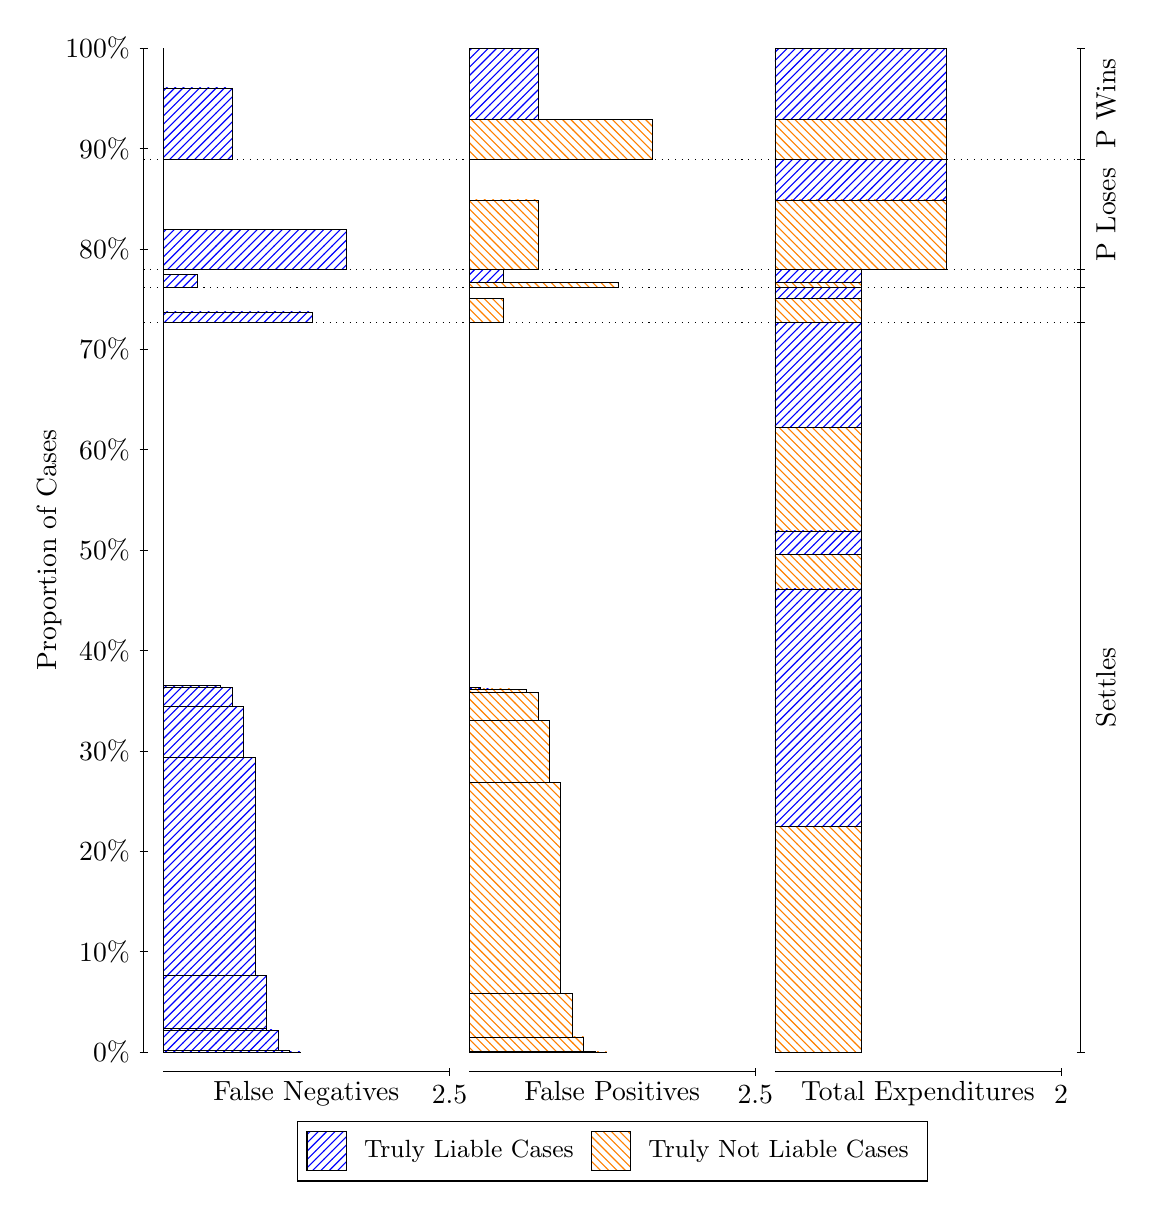
\begin{tikzpicture}
\draw[black, very thin] (1.5,1.75) -- (1.5,14.5);
\node[rotate=90, text=black, anchor=center] at (0.3, 8.125) {Proportion of Cases};
\draw[black, very thin] (1.45,1.75) -- (1.55,1.75);
\node[text=black, anchor=east] at (1.45, 1.75) {0\%};
\draw[black, very thin] (1.45,3.025) -- (1.55,3.025);
\node[text=black, anchor=east] at (1.45, 3.025) {10\%};
\draw[black, very thin] (1.45,4.3) -- (1.55,4.3);
\node[text=black, anchor=east] at (1.45, 4.3) {20\%};
\draw[black, very thin] (1.45,5.575) -- (1.55,5.575);
\node[text=black, anchor=east] at (1.45, 5.575) {30\%};
\draw[black, very thin] (1.45,6.85) -- (1.55,6.85);
\node[text=black, anchor=east] at (1.45, 6.85) {40\%};
\draw[black, very thin] (1.45,8.125) -- (1.55,8.125);
\node[text=black, anchor=east] at (1.45, 8.125) {50\%};
\draw[black, very thin] (1.45,9.4) -- (1.55,9.4);
\node[text=black, anchor=east] at (1.45, 9.4) {60\%};
\draw[black, very thin] (1.45,10.675) -- (1.55,10.675);
\node[text=black, anchor=east] at (1.45, 10.675) {70\%};
\draw[black, very thin] (1.45,11.95) -- (1.55,11.95);
\node[text=black, anchor=east] at (1.45, 11.95) {80\%};
\draw[black, very thin] (1.45,13.225) -- (1.55,13.225);
\node[text=black, anchor=east] at (1.45, 13.225) {90\%};
\draw[black, very thin] (1.45,14.5) -- (1.55,14.5);
\node[text=black, anchor=east] at (1.45, 14.5) {100\%};

\draw[black, very thin] (13.4,1.75) -- (13.4,14.5);
\draw[black, very thin] (13.35,1.75) -- (13.45,1.75);
\node[anchor=west] at (13.35, 1.75) {};
\draw[black, very thin] (13.35,11.013) -- (13.45,11.013);
\node[anchor=west] at (13.35, 11.013) {};
\draw[black, very thin] (13.35,11.46) -- (13.45,11.46);
\node[anchor=west] at (13.35, 11.46) {};
\draw[black, very thin] (13.35,11.684) -- (13.45,11.684);
\node[anchor=west] at (13.35, 11.684) {};
\draw[black, very thin] (13.35,13.085) -- (13.45,13.085);
\node[anchor=west] at (13.35, 13.085) {};
\draw[black, very thin] (13.35,14.5) -- (13.45,14.5);
\node[anchor=west] at (13.35, 14.5) {};

\draw[black, very thin, pattern color=blue, pattern=north east lines] (1.75,1.75) rectangle (3.494,1.7522);
\draw[black, very thin, pattern color=blue, pattern=north east lines] (1.75,1.7522) rectangle (3.3487,1.7721);
\draw[black, very thin, pattern color=blue, pattern=north east lines] (1.75,1.7721) rectangle (3.2033,2.0299);
\draw[black, very thin, pattern color=blue, pattern=north east lines] (1.75,2.0299) rectangle (3.058,2.0478);
\draw[black, very thin, pattern color=blue, pattern=north east lines] (1.75,2.0478) rectangle (3.058,2.7258);
\draw[black, very thin, pattern color=blue, pattern=north east lines] (1.75,2.7258) rectangle (2.9127,5.4873);
\draw[black, very thin, pattern color=blue, pattern=north east lines] (1.75,5.4873) rectangle (2.7673,6.1431);
\draw[black, very thin, pattern color=blue, pattern=north east lines] (1.75,6.1431) rectangle (2.622,6.3808);
\draw[black, very thin, pattern color=blue, pattern=north east lines] (1.75,6.3808) rectangle (2.4767,6.4014);
\draw[black, very thin, pattern color=blue, pattern=north east lines] (1.75,6.4014) rectangle (2.3313,6.4033);
\draw[black, very thin, pattern color=orange, pattern=north west lines] (1.75,6.4033) rectangle (1.75,11.013);
\draw[black, very thin, pattern color=blue, pattern=north east lines] (1.75,11.013) rectangle (3.6393,11.15);
\draw[black, very thin, pattern color=orange, pattern=north west lines] (1.75,11.15) rectangle (1.75,11.46);
\draw[black, very thin, pattern color=blue, pattern=north east lines] (1.75,11.46) rectangle (2.186,11.624);
\draw[black, very thin, pattern color=orange, pattern=north west lines] (1.75,11.624) rectangle (1.75,11.684);
\draw[black, very thin, pattern color=blue, pattern=north east lines] (1.75,11.684) rectangle (4.0753,12.198);
\draw[black, very thin, pattern color=orange, pattern=north west lines] (1.75,12.198) rectangle (1.75,13.085);
\draw[black, very thin, pattern color=blue, pattern=north east lines] (1.75,13.085) rectangle (2.622,13.993);
\draw[black, very thin, pattern color=orange, pattern=north west lines] (1.75,13.993) rectangle (1.75,14.5);
\draw[black, very thin, pattern color=orange, pattern=north west lines] (5.6333,1.75) rectangle (7.3773,1.7516);
\draw[black, very thin, pattern color=orange, pattern=north west lines] (5.6333,1.7516) rectangle (7.232,1.7598);
\draw[black, very thin, pattern color=orange, pattern=north west lines] (5.6333,1.7598) rectangle (7.0867,1.9413);
\draw[black, very thin, pattern color=orange, pattern=north west lines] (5.6333,1.9413) rectangle (6.9413,2.4988);
\draw[black, very thin, pattern color=orange, pattern=north west lines] (5.6333,2.4988) rectangle (6.796,5.1714);
\draw[black, very thin, pattern color=orange, pattern=north west lines] (5.6333,5.1714) rectangle (6.6507,5.9584);
\draw[black, very thin, pattern color=orange, pattern=north west lines] (5.6333,5.9584) rectangle (6.5053,6.3159);
\draw[black, very thin, pattern color=orange, pattern=north west lines] (5.6333,6.3159) rectangle (6.36,6.3581);
\draw[black, very thin, pattern color=orange, pattern=north west lines] (5.6333,6.3581) rectangle (6.2147,6.3599);
\draw[black, very thin, pattern color=blue, pattern=north east lines] (5.6333,6.3599) rectangle (5.924,6.3619);
\draw[black, very thin, pattern color=blue, pattern=north east lines] (5.6333,6.3619) rectangle (5.7787,6.3825);
\draw[black, very thin, pattern color=blue, pattern=north east lines] (5.6333,6.3825) rectangle (5.6333,11.013);
\draw[black, very thin, pattern color=orange, pattern=north west lines] (5.6333,11.013) rectangle (6.0693,11.323);
\draw[black, very thin, pattern color=blue, pattern=north east lines] (5.6333,11.323) rectangle (5.6333,11.46);
\draw[black, very thin, pattern color=orange, pattern=north west lines] (5.6333,11.46) rectangle (7.5227,11.521);
\draw[black, very thin, pattern color=blue, pattern=north east lines] (5.6333,11.521) rectangle (6.0693,11.684);
\draw[black, very thin, pattern color=orange, pattern=north west lines] (5.6333,11.684) rectangle (6.5053,12.572);
\draw[black, very thin, pattern color=blue, pattern=north east lines] (5.6333,12.572) rectangle (5.6333,13.085);
\draw[black, very thin, pattern color=orange, pattern=north west lines] (5.6333,13.085) rectangle (7.9587,13.592);
\draw[black, very thin, pattern color=blue, pattern=north east lines] (5.6333,13.592) rectangle (6.5053,14.5);
\draw[black, very thin, pattern color=orange, pattern=north west lines] (9.5167,1.75) rectangle (10.607,4.6122);
\draw[black, very thin, pattern color=blue, pattern=north east lines] (9.5167,4.6122) rectangle (10.607,7.632);
\draw[black, very thin, pattern color=orange, pattern=north west lines] (9.5167,7.632) rectangle (10.607,8.071);
\draw[black, very thin, pattern color=blue, pattern=north east lines] (9.5167,8.071) rectangle (10.607,8.3688);
\draw[black, very thin, pattern color=orange, pattern=north west lines] (9.5167,8.3688) rectangle (10.607,9.6775);
\draw[black, very thin, pattern color=blue, pattern=north east lines] (9.5167,9.6775) rectangle (10.607,11.013);
\draw[black, very thin, pattern color=orange, pattern=north west lines] (9.5167,11.013) rectangle (10.607,11.323);
\draw[black, very thin, pattern color=blue, pattern=north east lines] (9.5167,11.323) rectangle (10.607,11.46);
\draw[black, very thin, pattern color=orange, pattern=north west lines] (9.5167,11.46) rectangle (10.607,11.521);
\draw[black, very thin, pattern color=blue, pattern=north east lines] (9.5167,11.521) rectangle (10.607,11.684);
\draw[black, very thin, pattern color=orange, pattern=north west lines] (9.5167,11.684) rectangle (11.697,12.572);
\draw[black, very thin, pattern color=blue, pattern=north east lines] (9.5167,12.572) rectangle (11.697,13.085);
\draw[black, very thin, pattern color=orange, pattern=north west lines] (9.5167,13.085) rectangle (11.697,13.592);
\draw[black, very thin, pattern color=blue, pattern=north east lines] (9.5167,13.592) rectangle (11.697,14.5);
\draw[black, dotted] (1.5,11.013) -- (13.4,11.013);
\draw[black, dotted] (1.5,11.46) -- (13.4,11.46);
\draw[black, dotted] (1.5,11.684) -- (13.4,11.684);
\draw[black, dotted] (1.5,13.085) -- (13.4,13.085);
\draw[black, very thin] (1.75,1.5) -- (5.3833,1.5);
\node[text=black, anchor=north] at (3.5667, 1.5) {False Negatives};
\draw[black, very thin] (5.3833,1.45) -- (5.3833,1.55);
\node[text=black, anchor=north] at (5.3833, 1.45) {2.5};

\draw[black, very thin] (5.6333,1.5) -- (9.2667,1.5);
\node[text=black, anchor=north] at (7.45, 1.5) {False Positives};
\draw[black, very thin] (9.2667,1.45) -- (9.2667,1.55);
\node[text=black, anchor=north] at (9.2667, 1.45) {2.5};

\draw[black, very thin] (9.5167,1.5) -- (13.15,1.5);
\node[text=black, anchor=north] at (11.333, 1.5) {Total Expenditures};
\draw[black, very thin] (13.15,1.45) -- (13.15,1.55);
\node[text=black, anchor=north] at (13.15, 1.45) {2};

\node[text=black, centered, rotate=90] at (13.72, 6.3816) {Settles};


\node[text=black, centered, rotate=90] at (13.72, 12.385) {P Loses};
\node[text=black, centered, rotate=90] at (13.72, 13.793) {P Wins};

\draw (7.449999999999999,1.5) node[draw=none] (baseCoordinate) {};
\begin{scope}[align=center]
        \matrix[scale=0.5, draw=black, below=0.5cm of baseCoordinate, nodes={draw}, column sep=0.1cm]{
            \node[rectangle, draw, minimum width=0.5cm, minimum height=0.5cm, pattern color=blue, pattern=north east lines] {}; &
            \node[draw=none, font=\small, text=black] (B) {Truly Liable Cases}; &
            \node[rectangle, draw, minimum width=0.5cm, minimum height=0.5cm, pattern color=orange, pattern=north west lines] {}; &
            \node[draw=none, font=\small, text=black] (B) {Truly Not Liable Cases}; \\
            };
\end{scope}

\end{tikzpicture}
\end{document}